\documentclass{hxc_cl}

\usepackage{comment}
\usepackage{amsmath}
\usepackage{listings}
\usepackage{tabularx}
\newcolumntype{Y}{>{\centering\arraybackslash}X}
\usepackage{xcolor}%,colortbl}
\definecolor{Blue1}{rgb}{0.35,0.66,0.68}
\definecolor{Blue2}{rgb}{0.57,0.58,0.95}
\definecolor{BlueD}{rgb}{0.20,0.21,0.47}
\definecolor{mygreen}{rgb}{0,0.6,0}
\lstset{language=C,%
	ndkeywords={printf},
	basicstyle=\small\ttfamily,%
	keywordstyle=\color{mygreen},%
	stringstyle=\color{orange},
	ndkeywordstyle=\color{blue},
	commentstyle=\color{red},
    breaklines=true}

\newcommand{\hex}{0\text{x}}

\begin{document}

\title{Introducción a los punteros en C}
\author{Piou}
\date{}
\maketitle
\begin{resumen}
En este documento se presentan las propiedades básicas del uso de punteros en el lenguaje C, para aquellos a los manuales más completos les producen demasiado respeto. Se incluyen ejemplos para visualizar el funcionamiento y facilitar la comprensión del contenido.
\end{resumen}

\begin{requisitos}
\begin{itemize}
\item Programación básica en C. No es necesario saber nada de punteros.
\end{itemize}
\end{requisitos}

\section{Introducción}
Este artículo está escrito a partir del original, que se puede encontrar en \texttt{www.hackxcrack.es}, por el mismo autor. La edición anterior tiene aproximadamente 5 años. He intentado escribirlo más correctamente, y eliminar algunas partes superfluas.

Los punteros en C/C++ es algo que a la gente le cuesta entender al principio. Durante los últimos años la gente se introduce en programación mediante lenguajes de muy alto nivel, que ocultan y oscurecen los mecanismos internos mediante los que el sistema funciona.

Esto puede ser bueno, y de hecho hay muchos campos en los que esos mecanismos son totalmente irrelevantes, y los lenguajes con una mera herramienta para algo distinto. Sin embargo, pienso que conocer esos mecanismos es importante, y da mucho poder sobre el sistema cuando se saben usar. 

Los punteros dan acceso a uno de esos mecanismos: nos permiten acceder y operar directamente sobre la memoria del ordenador. Esto por supuesto puede ser complicado y hay que tener en cuenta sutilezas relacionadas con el aspecto de la memoria, pero una vez que se controla, es muy útil, permitiendo diseñar programas muy eficientes y rápidos.

Cuando aprendí a programar, hace unos 9 años, por mi propia cuenta, lo hice en C. Cuando llegué a punteros lo leí por encima entendiendo lo que eran, pero al terminar me quedé igual que al principio, ¿y esto para qué sirve?

Cubriremos dos aspectos básicos, el primero qué son y qué hacen, y el segundo varias aplicaciones prácticas. A la hora de optimizar y diseñar algoritmos usando punteros, como con cualquier herramienta, cuanto más interiorizada la tengas, mejor la usarás. Por eso creo que es importante insistir en la necesidad de practicar, con cualquier cosa, por chorra que sea. Eso dará, además de práctica, mucho conocimiento sobre cómo se comportan las estructuras de memoria.

\section{Introducción a la memoria del ordenador}

Esta sección introduce conceptos básicos del funcionamiento de la memoria del ordenador.

La memoria, como sabrás, se organiza en bits. Los bits son la unidad de memoria más pequeña. Son objetos que pueden tomar dos valores, $0$ ó $1$. Para trabajar con algo más de comodidad, se usan bytes, que son agrupaciones de 8 bits. Se usan $8$ porque es un número lo suficientemente grande para considerarlo unidad de información (por ejemplo en la codificación ASCII cada letra o símbolo se puede almacenar en un byte) y porque al ser potencia de dos permite una conversión directa y sencilla con la base hexadecimal.

Esta memoria se almacena en el ordenador en varios lugares (lugares físicos). Cada lugar tiene una capacidad distinta y una velocidad de acceso distinta, como se representa en la figura \ref{fig:memoria}.

\begin{figure}[H]
\centering
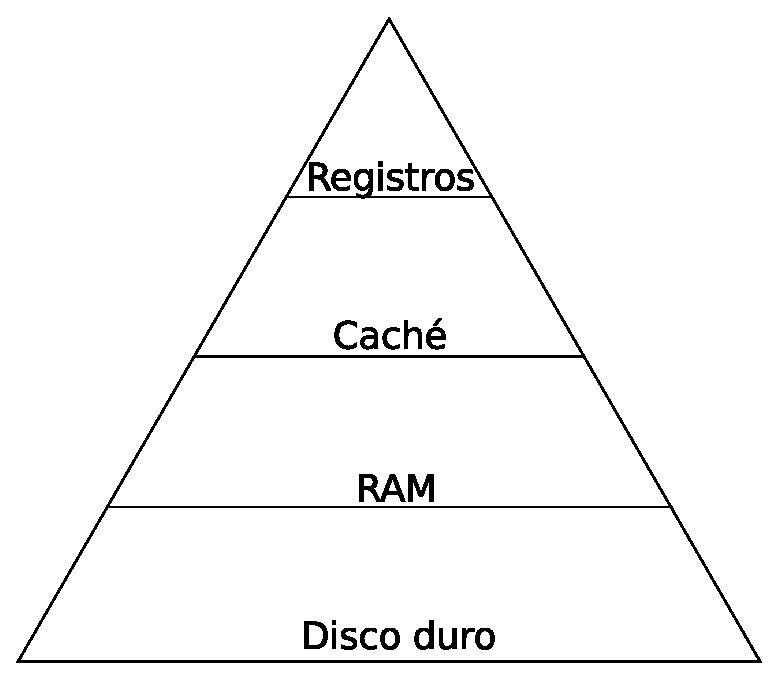
\includegraphics[width=5cm]{memoria}
\caption{\label{fig:memoria}Memoria de un ordenador. Más abajo en la pirámide implica mayor tamaño y más lentitud de acceso.}
\end{figure}

El disco duro permite una capacidad grande de almacenaje pero es lento acceder a él. La memoria RAM es mucho menor (tamaños típicos son entre $4$ y $8$ GB), pero es de acceso mucho más rápido que el disco duro. Los programas al ejecutarse se vuelcan desde donde están guardados (disco duro), a la memoria RAM, y se ejecutan desde allí.

La caché y los registros son zonas de memoria del procesador, de acceso muy rápido pero muy pequeñas. Los registros suelen tener sólo $32$ o $64$ bits, aunque el procesador tarda del orden de nanosegundos en acceder a la memoria de los registros.

En la memoria RAM (que nos interesa ahora), las direcciones de memoria se numeran en notación hexadecimal. Como hemos mencionado, la conversión entre binario y hexadecimal es muy sencilla. Se pueden transformar grupos de cuatro bits en una letra hexadecimal. Por ejemplo, el número binario $10010101111$ se puede separar en conjuntos de cuatro bits (empezando por la derecha): $100|1010|1111$. Y podemos convertir directamente directamente esos números a hexadecimal:
\begin{align*}
100_2&=4_{10}=4_{16}\\
1010_2&=10_{10}=A_{16}\\
1111_2&=15_{10}=F_{16}
\end{align*}
El subíndice indica la base numérica. El resultado sería, entonces, que $10010101111_2=4AF_{16}$.

Por último, hay que mencionar que, en C, los números hexadecimales se nombran poniendo delante 0x, así que en el documento de aquí en adelante nos referiremos a ellos así. El número anterior sería entonces $\hex4AF$.

Me he dejado un montón de aspectos sobre la memoria en el tintero, pero intento ser muy conciso. Creo que es mejor mancharse las manos un poco antes de profundizar más en el funcionamiento interno (que también es importante, y el lector interesado debería buscar más información).

Pasemos entonces a lo que hemos venido.

\section{¿Qué es un puntero?}
La manera más fácil de definir un puntero y que no echará a nadie para atrás es: un puntero es una variable, nada más que eso.

Tenemos muchos tipos de variables que cambian en lo que podemos meter dentro. Tenemos variables en las que podemos guardar números enteros (tipo \texttt{int}), números en coma flotante (tipos \texttt{float, double}), letras (tipo \texttt{char}), etc. ¿Y qué podemos meter en un puntero? Algo tan simple como una dirección de memoria. ¿Y eso qué es?

Vamos a ver un poco cómo funciona la memoria del ordenador. Quizás no te hayas planteado qué pasa cuando defines una variable. Cuando escribimos:

\begin{lstlisting}
int numero = 5;
\end{lstlisting}

¿Qué hace el ordenador? Cuando compilamos el programa, el compilador traduce nuestro código a código máquina. El código máquina son sentencias que el procesador puede ejecutar directamente. El ejecutable que produce el compilador es una sucesión lineal de este tipo de sentencias, nada más.

Cuando lo ejecutamos, el ordenador vuelca el contenido en la RAM, separando el código en varias zonas.  Hay una zona en la que se guardan las sentencias que se ejecutarán. En otra zona se almacenan las variables. Esta zona se reserva por el sistema para el programa en cuestión.

En resumen, cuando escribimos algo como lo anterior el sistema reservará la memoria necesaria para almacenar esa variable. La cantidad de memoria que reserve depende del tipo de variable, y la función \texttt{sizeof} devuelve este dato. Si hacemos:

\begin{lstlisting}
int numero;
printf("Tamaño de int: %i\n",sizeof(int));
\end{lstlisting}

el programa mostrará: \textit{Tamaño de int: 4}. La variable \texttt{int} ocupa $4$ bytes $=32$ bits.

Podemos ver la memoria RAM como una tabla, o una lista de direcciones, en la que podemos meter cosas. Estas direcciones, como dije en la introducción, se numeran de manera hexadecimal, es decir, con numéros del $0$-$F$.

Supongamos que tenemos la memoria de la siguiente manera:

\begin{center}
% BEGIN RECEIVE ORGTBL memoria1
\begin{tabular}{cc}
{\bf Dirección} & {\bf Contenido} \\
%\rowcolor{Blue1}
$\hex00000001$ & - \\
%\rowcolor{Blue2}
$\hex00000002$ & - \\
%\rowcolor{Blue1}
$\hex00000003 $ & - \\
%\rowcolor{Blue2}
$\hex00000004  $ & - \\
%\rowcolor{Blue1}
$\hex00000005   $ & - \\
%\rowcolor{Blue2}
$\hex00000006   $ & - \\
\end{tabular}
% END RECEIVE ORGTBL memoria1
\begin{comment}
#+ORGTBL: SEND memoria1 orgtbl-to-latex :splice nil :skip 0
| {\bf Dirección}   | {\bf Contenido} |
| $\hex00000001$    | -               |
| $\hex00000002$    | -               |
| $\hex00000003 $   | -               |
| $\hex00000004  $  | -               |
| $\hex00000005   $ | -               |
| $\hex00000006   $ | -               |
\end{comment}
\end{center}

Ahora, en nuestro programa ponemos la definición de una variable tipo \texttt{char}, que se llame, por ejemplo, \texttt{caracter}, y que como sabemos, ocupa un byte en memoria.

\begin{lstlisting}
char caracter;
\end{lstlisting}

Al hacer lo anterior, el ordenador nos reserva en la memoria el espacio necesario para esa variable. El lugar concreto en la memoria depende de tantos factores que podemos decir que es aleatorio. Supongamos que le reserva la posición $\hex00000002$. La variable \texttt{char} la podemos ver como un entero entre $0$ y $255$, o entre $-127$ y $-128$, dependiendo de si es \texttt{signed} o \texttt{unsigned}.

Como hemos vsto: $1\text{ byte}=8\text{ bits}$. En binario, ocho bits comopletos $11111111_2=256_{10}$, que es el máximo número que podemos guardar ahí.

Cuando el ordenador reserve la memoria, la tabla quedará así (la letra en negrita significa que el espacio está reservado):

\begin{center}
\begin{tabular}{cc}
{\bf Dirección} & {\bf Contenido} \\
%\rowcolor{Blue1}
$\hex00000001$ & - \\
%\rowcolor{Blue2}
\bf$\mathbf{\hex00000002}$ & - \\
%\rowcolor{Blue1}
$\hex00000003 $ & - \\
%\rowcolor{Blue2}
$\hex00000004  $ & - \\
%\rowcolor{Blue1}
$\hex00000005   $ & - \\
%\rowcolor{Blue2}
$\hex00000006   $ & - \\
\end{tabular}
\end{center}

Ahora le damos un valor a la variable, por ejemplo la letra \texttt{m}.

\begin{lstlisting}
caracter = 'm';
\end{lstlisting}

El código ASCII de la letra \texttt{m} minúscula es el $109=\hex6D$, así que al asignar el valor, la memoria quedará así:

\begin{center}
\begin{tabular}{cc}
{\bf Dirección} & {\bf Contenido} \\
%\rowcolor{Blue1}
$\hex00000001$ & - \\
%\rowcolor{Blue2}
\bf$\mathbf{\hex00000002}$ & $\mathbf{\hex6D}$ \\
%\rowcolor{Blue1}
$\hex00000003 $ & - \\
%\rowcolor{Blue2}
$\hex00000004  $ & - \\
%\rowcolor{Blue1}
$\hex00000005   $ & - \\
%\rowcolor{Blue2}
$\hex00000006   $ & - \\
\end{tabular}
\end{center}

\section{Funcionamiento de los punteros}

Siguiendo con lo que tenemos, vamos a usar un puntero para apuntar a esa variable.

El uso de punteros es ligeramente distinto al de variables corrientes. Para definir un puntero lo hacmeos igual que ocn una variable, pero usando un asterisco entre el tipo de puntero y el nombre del puntero.

Vamos a definir un puntero que apunte a la variable \texttt{caracter}, y que se llame \texttt{ptr}. De momento sólo lo definimos:

\begin{lstlisting}
char *ptr;
\end{lstlisting}

Supongamos que el ordenador le reserva espacio a la variable \texttt{ptr} justo después de la variable \texttt{caracter}. La memoria quedará:

\begin{center}
\begin{tabular}{cc}
{\bf Dirección} & {\bf Contenido} \\
$\hex00000001$ & - \\
\bf$\mathbf{\hex00000002}$ & $\mathbf{\hex6D}$ \\
\bf$\mathbf{\hex00000003} $ & - \\
\bf$\mathbf{\hex00000004}  $ & - \\
\bf$\mathbf{\hex00000005}   $ & - \\
\bf$\mathbf{\hex00000006}   $ & - \\
\end{tabular}
\end{center}

Ahora le damos un valor. ¿Cómo le damos la posición de memoria de la variable \texttt{caracter}? Esto se hace con el operador \&. Cuando ponemos este operador delante de una variable lo que hace es devolver su dirección de memoria, en vez de su valor. Para hacer que \texttt{ptr} apunte a \texttt{caracter}, hacemos:

\begin{lstlisting}
ptr = &caracter;
\end{lstlisting}

Fácil, ¿no? Más tarde explicaré cuándo usar el * para un puntero y cuándo no. Pero antes, ¿cómo queda ahora la tabla de memoria? Es fácil imaginarlo:

\begin{center}
\begin{tabular}{cc}
{\bf Dirección} & {\bf Contenido} \\
$\hex00000001$ & - \\
\bf$\mathbf{\hex00000002}$ & $\mathbf{\hex6D}$ \\
\bf$\mathbf{\hex00000003} $ & \bf$\mathbf{\hex00000002}$ \\
\bf$\mathbf{\hex00000004}  $ & - \\
\bf$\mathbf{\hex00000005}   $ & - \\
\bf$\mathbf{\hex00000006}   $ & - \\
\end{tabular}
\end{center}

¿Quedará así? ¿Seguro? Pues no. ¿Cómo se organizaba la memoria? En bytes. ¿Y cuántas hexadecimales puede tener un byte? $1\text{ byte}=8\text{ bits}$. $1$ Cifra hexadecimal por cada $4$ bits implica que $1$ byte puede almacenar $2$ dígitos hexadecimales.

Las posiciones en memoria ocupan $8$ cifras hexadecimales, que son $4$ bytes, así que necesitaremos cuatro posiciones, tal y como el sistema nos había reservado. La tabla quedará así:

\begin{center}
\begin{tabular}{cc}
{\bf Dirección} & {\bf Contenido} \\
$\hex00000001$ & - \\
\bf$\mathbf{\hex00000002}$ & $\mathbf{\hex6D}$ \\
\bf$\mathbf{\hex00000003} $ & \bf$\mathbf{\hex00}$ \\
\bf$\mathbf{\hex00000004}  $ &  \bf$\mathbf{\hex00}$\\
\bf$\mathbf{\hex00000005}   $ & \bf$\mathbf{\hex00}$\\
\bf$\mathbf{\hex00000006}   $ & \bf$\mathbf{\hex02}$ \\
\end{tabular}
\end{center}

Un puntero siempre ocupa la misma memoria para un sistema concreto. Si la memoria se numera como aquí, es decir, en cuatro bytes, entonces los punteros ocuparán lo suficiente como para almacenar $4$ bytes, es decir, $4$ bytes.

Es importante tener en cuenta que un puntero siempre ocupa lo mismo, independientemente del tipo de variable al que apunte.

En este punto ya tenemos la memoria como en la anterior tabla, con dos variables: una tipo \texttt{char} con la letra \texttt{m} y un puntero \texttt{ptr} que apunta a la primera. Veamos ahora cómo usar esto.

Al definir el puntero vimos que se hacía con un asterisco *. Esto es siempre necesario al definir un puntero. Si ponemos un asterisco al definir una variable, esto se entenderá como un puntero que apuntará a una variable del tipo que le hayamos puesto. Pero vemos también que apuntara a la variable \texttt{caracter} (\texttt{puntero=\&caracter}), no se usó el asterisco. ¿Cuándo se usa y cuándo no?

Hay multitud de usos de un puntero, en algunos casos se ha de usar el asterisco y en otros no, así que para saber  si debemos usarlo, mejor que aprender casos concretos, que es imposible, aprenderemos la regla general:

{\bf Siempre que definamos un puntero se usa un asterisco *.

Cuando lo usamos (después de definirlo), NO poner un asterisco significa usar su contenido, es decir, la dirección de memoria a la que apunta; y usar el asterisco significa acceder al valor de la dirección de memoria a la que apunta.}

Entederemos esto mejor con un ejemplo. Retomamos el caso anterior. Tenemos una variable \texttt{caracter}, con el valor \texttt{m} en la posición $\hex00000002$; y una variable \texttt{ptr} con el valor $\hex00000002$, es decir, apuntando a la variable \texttt{caracter}, tal y como está en la última tabla.

Si nos referimos a la variable \texttt{ptr} sin el asterisco, nos estamos refiriendo, según la regla, a la dirección que ocupa. En realidad esto es como con cualquier otra variable. Cuando pones una variable, por ejemplo tipo \texttt{int}, lo que estás cambiando es su valor. Por ejemplo:

\begin{lstlisting}
int numero = 5;
numero = 10;
\end{lstlisting}

Al poner \texttt{numero} nos referimos a su valor ($5$), y lo cambiamos a $10$. En un puntero es igual, si lo pones tal cual, a lo que te refieres es a su valor, y el valor de un puntero es la dirección a la que apunta. Si hacemos:

\begin{lstlisting}
printf("Dirección: %p\n", ptr);
//El %p significa que le pasamos un puntero
\end{lstlisting}

nos mostrará el contenido de \texttt{ptr}, que es la dirección a la que apunta: $\hex00000002$.

El asterisco, según la regla, es el contenido de la dirección a la que apunta el puntero. Puesto que apunta a un \texttt{char}, ponerlo con asterisco significa acceder al valor del \texttt{char}. Por ejemplo, si queremos cambiar el contenido de la variable \texttt{caracter}, que tiene una \texttt{m}, por una \texttt{c}, y lo queremos hacer a través de \texttt{ptr}, haremos:

\begin{lstlisting}
*ptr = 'c';
\end{lstlisting}

El asterisco significa que accedemos al contenido de la dirección de memoria $\hex00000002$, y lo cambiamos por una \texttt{c}, cuyo valor hexadecimal en ASCII es el $\hex63$. La tabla quedará así:

\begin{center}
\begin{tabular}{cc}
{\bf Dirección} & {\bf Contenido} \\
$\hex00000001$ & - \\
\bf$\mathbf{\hex00000002}$ & $\mathbf{\hex63}$ \\
\bf$\mathbf{\hex00000003} $ & \bf$\mathbf{\hex00}$ \\
\bf$\mathbf{\hex00000004}  $ &  \bf$\mathbf{\hex00}$\\
\bf$\mathbf{\hex00000005}   $ & \bf$\mathbf{\hex00}$\\
\bf$\mathbf{\hex00000006}   $ & \bf$\mathbf{\hex02}$ \\
\end{tabular}
\end{center}

Creo que con esto ha quedado bastante claro el uso del asterisco, en cada caso particular tenemos que ver si interesa usar la dirección de memoria o nos interesa el valor almacenado en la dirección a la que apunta.

La siguiente parte de este texto intenta justificar la razón por la que hay que definir el puntero con el tipo de la variable a la que apunta (porqué definíamos el puntero como \texttt{char *ptr}).

¿Por qué hay que darle entonces el mismo tipo que la variable? La respuesta es simple. Las variables, independientemente del tipo, siempre contienen lo mismo vistas en memoria: un número hexadecimal. Lo que cambia es (a parte de la manera en la que el lenguaje las interpreta) el espacio que ocupa. Vamos a ver el problema con un ejemplo. Supongamos que tenemos una variable \texttt{int} que ocupa $4$ bytes ($32$ bits). Como $2$ cifras hexadecimales representan un byte completo, tenemos $8$ cifras hexadecimales. La variable tiene guardado el número $\hex98FC3F4A$. Los bytes, por razones de la estructura de la pila, algo que ahora no interesa, se guardan en sentido inverso, así que el número quedará en memoria así:

\hspace{-0.5cm}\begin{tabularx}{0.48\textwidth}{|Y|Y|Y|Y|}
\hline 4A & 3F & FC & 98 \\ \hline
\end{tabularx}

Ahora creamos un puntero que apunte a la variable. Tenemos un descuido y envez de definirlo tipo \texttt{int *} lo definimos tipo \texttt{char *}. El programa pensará que, al ser un puntero tipo \texttt{char}, está apuntando a una variable tipo \texttt{char}, es decir, a un byte. Osea que se quedará en tan solo el primer byte (4A).

Si cambiamos el valor de la variable a través del puntero, sólo afectará al último byte (por ser el primero en la memoria, ya que piensa que la variable a la que apunta sólo ocupa un byte. Si, por ejemplo, le damos el valor de $\hex 43$ a través adel puntero, la variable pasará a ser $\hex 98FC3F43$, en vez de $\hex 00000043$.

Puedes comprobar el efecto compilando y ejecutando este programa:

\begin{lstlisting}
#include <stdio.h>

int main() {
  int numero = 0x98fc3f4a;
  char *puntero_malo = \& numero;

  printf("Número original: %#X\n",numero);
  printf("Número desde puntero original: %#X\n",*puntero_malo);

  *puntero_malo = 0x43;

  printf("Número: %#X\n", numero);
  printf("Número desde puntero: %#X\n", *puntero_malo);

  return 0;
}
\end{lstlisting}

En mi ordenador, la salida del programa es:

\begin{lstlisting}
Numero original: 0x98FC3F4A
Numero desde puntero original: 0x4A
Numero: 0x98FC3F43
Numero desde puntero: 0x43
\end{lstlisting}

Esta es la razón por la que a los punteros se les tiene que asignar el mismo tipo que a las variables a las que apunten. El sistema debe saber el tamaño de la información a la que está accediendo.

No dejes que todo esto de los bytes que se guardan al revés te líe, quédate con la teoría de cómo funciona un puntero y para empezar es suficiente.

\section{Cuidados a tener en cuenta}

Como todo en esta vida, los punteros tienen también sus inconvenientes, y es que manejar directamente la memoria puede ser ``peligroso''. Los fallos de programación originados por un mal uso de punteros suelen ser a menudo los más difíciles de encontrar y corregir (en realidad sobre todo de encontrar). En esta parte veremos algunos cuidados que tenemos que llevar a cabo a la hora de usar punteros.

Como dijimos al principio del documento, el ordenador vuelca en la RAM los programas que ejecuta. Cuando un programa se libera de la memoria, es decir, cuando lo cerramos, la memoria que ocupaba pasa a ser memoria libre disponible para un nuevo programa. La información que tenía, sin embargo, no tiene por qué borrarse.

Esto quiere decir que si definimos una variable y no le damos un valor, esta variable tendrá lo que tuviera la zona de memoria que se reservó cuando fue usada por otro programa o por el sistema operativo, es decir, es imposible saber lo que tiene una variable si no le asignamos un valor inicial. Prueba a ejecutar el siguiente programa:

\begin{lstlisting}
#include <stdio.h>

int main() {
  int number;
  printf("Número: %i\n",number);
  return 0;
}
\end{lstlisting}

Si lo ejecutas varias veces verás que te dará una serie de números que desde luego, no son $0$, y que son distintos entre sí. Esto ocurre porque hemos definido la variable, el ordenador le ha reservado un hueco en memoria, pero no hemos guardado nada en ese hueco, no sabemos qué hay.

Este problema con las variables no tiene mucha relevancia porque con las variables sólo modificamos el contenido de la variable, y esa zona de la memoria ya pertenece a nuestro programa, por lo que cualquier cambio es legítimo y no surgirán problemas. ¿Pasa lo mismo con los punteros?

Si definimos un puntero pero no hacemos que apunte a ninguna variable:

\begin{lstlisting}
int *puntero;
\end{lstlisting}

El contenido de la variable \texttt{puntero} puede contener cualquier valor, y ese valor, puesto que es un puntero, será interpretada como una dirección de memoria. Tenemos una variable con una dirección de memoria aleatoria. Esto supone un problema muy grande. Si ahora hacemos:

\begin{lstlisting}
*puntero = 5;
\end{lstlisting}

Estamos diciendo que la variable a la que apunte valga $5$, pero el puntero está apuntando a una dirección que no conocemos. Podría estar sobreescribiendo cualquier cosa, incluso memoria que esté ocupando el sistema operativo para algo esencial en su funcionamiento, lo que podría provocar un ``cuelgue''.

Este problema se encuentra presenta sobre todo en Windows. Puede probar a hacer eso, y si lo haces muchas veces quizás el ordenador se cuelgue alguna de ellas y lo tengas que reiniciar. En sistemas GNU/Linux el sistema avisa de una ``violación de segmento'' y cierra el programa cuando se intenta escribir en memoria prohibida.

Esta sección se resume en esto: cuidado cuando uses un puntero, ten en cuenta a dónde apunta y que siempre tenga un valor conocido.

En la sección siguiente explicaré cuidados concretos que hay que tener para los usos que doy, aunque sabiendo esto deberías ser capaz de suponerlos.

\section{Algunos usos}

Sería inútil intentar enumerar todos los usos que tienen los punteros. Tienen virtualmente infinitos. Aquí pondré algunos comunes con ejemplos para que puedas practicar y acostumbrar a usarlos. Los punteros son sin duda el punto fuerte de C. Te permiten un control mucho más a fondo del ordenador, un control directo de la memoria que se puede aprovechar de mil y una maneras, y depende de ti el saber aprovecharlos en cada situación.

\subsection{Pasar argumentos por referencia. (Sólo en C, no en C++)}

Cuando creamos una función podemos ponerle argumentos, una serie de datos con los que la función puede trabajar, pero C siempre pasa esos argumentos por valor. Esto significa que cuando pasamos una variable como el argumento a una función, lo que hace el programa es pasarle a la función una copia del valor de la variable, sin cambiar la variable. Si por ejemplo tenemos la siguiente función:

\begin{lstlisting}
int suma(int a, int b) {
  a += b;
  return a;
}
\end{lstlisting}

Cuando le pasemos una variable a los argumentos se pasará sólo su valor, quedando la variable intacta. si hacemos por ejemplo:

\begin{lstlisting}
int numero1 = 5;
int numero2 = 10;
int numero3 = suma(numero1,numero2);
\end{lstlisting}

A pesar de que dentro de la función a la variable \texttt{a} se le sume la variable \texttt{b}, la variable \texttt{numero1} no sufre ningún cambio, esto es evidente.

¿Qué pasa si queremos que la variable \texttt{numero1} sí que sufra los cambios que se le hacen dentro de la función? En principio no podemos, porque sólo le estamos pasando el valor de la variable, y por lo tanto sólo podemos pasar valores, no la variable en sí.

Pero tenemos nuestros maravillosos punteros. Una solución al problema es pasarle la dirección de memoria de la variable \texttt{numero1}, de modo que dentro de la función tenemos la dirección de memoria en la que está guardada esa variable, y podemos modificarla directamente. Para ello habrá que especificar el primer argumento como un puntero, ya que le pasaremos una dirección de memoria y no un número entero. La función queda:

\begin{lstlisting}
int suma(int *a, int b) {
  *a += b;
  return *a;
}
\end{lstlisting}

El argumento lo definimos como puntero poniéndole un asterisco. Dentro de la función, puesto que nos referimos al valor de la dirección a la que apunta, también usamos el asterisco. La función se usaría así;

\begin{lstlisting}
int numero1 = 5;
int numero2 = 10;
int numero3 = suma(&numero1, numero2);
//Aquí la variable numero1 valdrá 15 ya que la hemos cambiado dentro de la función
\end{lstlisting}

Como el argumento es un puntero a \texttt{int}, le tenemos que pasar la dirección de memoria de la variable, que se hace, como ya vimos, con el operador \&.

En el título de la subsección he puesto que esto es para C y no C++. En realidad se puede usar igual en C++, pero no es necesario porque C++ ya tiene un sistema de paso de argumentos por referencia a funciones, que se hace defininiendo los argumentos con el símbolo \&, y pasando la variable de manera normal. Eso no compete a este documento.

\subsection{Recorrer arrays}

Este es otro uso bastante importante y común.

Supongamos que tenemos un array de variables \texttt{int} formado por $100$ elementos:

\begin{lstlisting}
int numeros[100];
\end{lstlisting}

Antes de seguir hay que hacer una aclaración. Los arrays y los punteros son similares en uso. Si nos referimos a un array poniendo sólo su nombre, sin especificar el índice, lo que nos va a devolver será la dirección de memoria del primer elemento, es decir, es lo mismo poner \texttt{numeros} que \texttt{\&numeros[0]}. Y es importante saber para entender esto que los elementos de un array están colocados de manera lineal en la memoria, todos seguido y en orden.

Podemos recorrer un array si creamos un puntero \texttt{int} y hacemos que apunte al primer elemento.

\begin{lstlisting}
int *puntero = numeros;
//Sería lo mismo que poner:
//int *puntero = \&numeros[0];
\end{lstlisting}

\end{document}
